\documentclass{article}


%\usepackage{nips_2017}
\usepackage[final]{nips_2017}
% to compile a camera-ready version, add the [final] option, e.g.:
% \usepackage[final]{nips_2017}

\usepackage[utf8]{inputenc} % allow utf-8 input
\usepackage[T1]{fontenc}    % use 8-bit T1 fonts
\usepackage{hyperref}       % hyperlinks
\usepackage{url}            % simple URL typesetting
\usepackage{booktabs}       % professional-quality tables
\usepackage{amsfonts}       % blackboard math symbols
\usepackage{nicefrac}       % compact symbols for 1/2, etc.
\usepackage{microtype}      % microtypography
\usepackage[super]{nth}     % JK: for 1st-ing and 2nd-ing
\usepackage{graphicx}       % added by seth - image support
\graphicspath{ {./images/} }
\usepackage{soul}           % added by seth - remove before submission, provides highlighting support

\usepackage{hyperref}
\hypersetup{
    colorlinks=true,
    linkcolor=blue,
    filecolor=magenta,      
    urlcolor=blue,
}
 
\urlstyle{same}
\title{%
  Kung Faux Pandas \\
  \large Alternative Facts for Privacy Protection}

\author{
  James King \& Seth Russell\\
  Data Science to Patient Value (D2V)\\
  School of Medicine \\
  University of Colorado Anschutz Medical Campus\\
  Aurora, CO\\
  \texttt{james.king@ucdenver.edu} \\
  \texttt{seth.russell@ucdenver.edu} \\
  }

\date{May 2018}

\begin{document}

% Advice from Tell:  articulate the problem with evidence (i.e. papers)
%   Enable reproducibility - patient value, make process of replication easier
%   Time saving
%   legal risk (carrying data in laptops, etc)
%   Multiple comparison?
%   Educational data sets
%  Definition of :reproducibility 
%       reproducibilty - everything same - code, data, result
%       replicability - code same, new data, same result find Peng & Leek reference (also look at blog)
%   unit testing...
%   Proof of privacy guarantees?

\makeatletter

\newenvironment{chapquote}[2][2em]
  {\setlength{\@tempdima}{#1}%
   \def\chapquote@author{#2}%
   \parshape 1 \@tempdima \dimexpr\textwidth-2\@tempdima\relax%
   \itshape}
  {\par\normalfont\hfill--\ \chapquote@author\hspace*{\@tempdima}\par\bigskip}
\makeatother

\maketitle

\begin{abstract}
\hl{to finish:} A description of an end-to-end system for easily generating synthetic data which contains no Personal Health Information (PHI), allowing example data to be distributed for reproducibility testing and other purposes.  

\end{abstract}


\section{Introduction}

%Reproducing machine learning results in the field of health care is challenging. Many published research articles do not make code nor data available which limits the ability of others to reproduce results. While journals could require the inclusion of code and data in submissions, there are legal restrictions that prevent the sharing of data in the health care domain \cite{hippapro}.

%There are various approaches to building data sets which simultaneously have scientific utility and comply with privacy laws. Broadly speaking, these methods fall into two categories: anonymization and synthesis. Anonymization methods attempt to keep as much of the "real" data as possible, whilst ensuring that person-specific data is generalized so distributed data cannot be tied to a single individual. Synthetic methods generate data based on algorithms, publicly known disease models, or other sources not specific to an individual.

%The unique contribution to the space of reproducible machine learning by this paper is a no-configuration required method for faux-data creation from user generated queries. The faux-data will resemble the original data set but can be used freely without compliance risk because it contains no Protected Health Information (PHI). Furthermore, with this method it is possible for an investigator to perform hypothesis articulation, data cleaning, analysis, visualization, and documentation without the ever having access to the underlying PHI data.

\begin{chapquote}{Richard Dawkins on his preference for the scientific method over other modes of inquiry.}
``Because it works, bitches.''
\end{chapquote}

The ability of independent investigators to verify results is perhaps \emph{the} most fundamental feature that separates science from other forms intellectual inquiry.  Unfortunately, the mechanisms of communicating scientific results have changed little since the age of enlightenment and are inadequate enabling reproducibility for some modern scientific endeavors such as machine learning.  Perhaps the most important impediment to reproducibility is the need to share data.  This has long been difficult in health care fields, but will presently become difficult for just about everyone.

There is a large body of published literature detailing methods for overcoming this difficulty via ``anonymizing'' and ``synthesising'' data \cite{<give the bigguns>}, however at present a mechanism to routinely \emph{use} these techniques has not been forthcoming.

This paper details an open source software library called \emph{Kung Faux Pandas (KFP)} which integrates \emph{any} of these data security methods into the popular Python Pandas data science library. For those who prefer other tools, KFP also provides Structured Query Language (SQL) interface which enables users to arbitrarily query any data within a database, returning to the user a data set which either does not contain any personal information (synthesized) or has been anonymized by standard methods.

\section{Background}

Machine Learning (ML) methods are perhaps the most difficult to make ``reproducible'' in any sense of the term.   This difficulty has many sources:  a quickly evolving set of software tools with various levels of compatibility, a need for massive computational infrstructure, the ``black magic'' methods for building the model structures, and intense apetite for training data.   Huge piles of training data.

So in order to reproduce a model, one needs a full set of library metadata, an impossibly expensive computer, model metadata which is nearly impossible to replicate by a description, and a large data set that the original researchers are not likely to give you.  

The first few of those obstacles are technological in nature and can be overcome by some subtle alterations in the ``scientific machine'' and improvements to computing.   That last problem, though, is HUGE.  A reproducer needs appropriate data, even to simply veryify that a trained model actually works as described.   Setting aside the natural tendency of scientists to dislike sharing data out of fear of being scooped, there are ominous legal constraints on data sharing which will most likely become more intense over time.

At the writing of this paper, the European Union's (EU) General Data Protection Regulation (GDPR) has come into full effect \cite{<get the text of the rules cided>}, extending the preeminance of data privacy over data sharing to all fields in that jurisdiction.   In fact, the GDPR enables the data owner (i.e. the person about whom the data is collected) has the ability to revoke permission to use the data at any time. Most other countries will likely implement similar legislation in the near future \cite{?}.

Thus, without signifcant technological and policy infrastructure, it's essentially illegal to share data about humans.  By extension, it's difficult if not outright illegal to attempt to reproduce the results of a machine learning model created by an outside entity.




%Though there are semantic variations in the use of the words "replicate," "reproduce," etc., most commentaries on the subject agree that an independent experiment with confirmatory results is the strongest support of any experiment \cite{leek_opinion_2015, drummond_replicability_2009}.  In the machine learning context, the ability to independently arrive at similar results from similar data requires the documentation of many technical (and frankly, banal) parameters which is rarely done within published papers.  Many of these, such as the versions used of various software libraries, can be captured in virtual environments, but parameters related to the data are often much trickier to capture, particularly if the data used in an analysis is sensitive and cannot be shared.



%\subsection{Seth's Original}
%Over the past 18 years, there has been several significant papers clarifying the definition and importance of reproducibility along with the closely related term replicability. Leek and Peng have defined reproducibility as the "ability to recompute data analytic results given an observed dataset and knowledge of the data analysis pipeline," and replicability as "the chance that an independent experiment targeting the same scientific question will produce a consistent result" \cite{leek_opinion_2015}; others such as Drummond use the terms in a reverse fashion \cite{drummond_replicability_2009}. Despite the semantic disagreement, both groups agree that an independent experiment with confirmatory results is the strongest support of any experiment. One early influential paper on the topic of reproducibility in scientific computing details key factors in reproducibility as having: data, input parameters, documentation, software code, and an environment capable of running the provided software code; items that cannot easily nor clearly be communicated by paper \cite{schwab_making_2000}. Reproducibility should be treated as a minimum required standard that all published research should meet \cite{peng_reproducible_2006}. Specifically in the context of machine learning, this means including details to a level someone else could create the same environment including hardware configuration and run times, data used for all experiments, source code, documentation on data and how to run/configure software, and tests that verify the software runs correctly. The last item is important but often overlooked - unit tests can show how a researcher validated their code was giving expected results which can often lead to insights not normally communicated in a results section of a journal article. Once a result can be reproduced, new researchers can then build upon the methods, gather new data for testing/validation, or discover alternative methods to replicate a result.

%As machine learning results are highly data dependent, the barriers around sharing health data make it difficult or impossible for others to verify or reproduce results with novel machine learning methods in the health care domain (? cite recent difficult to reproduce examples such as Google FHIR paper, others?). In order to resolve the problem of data sharing, various methods for data synthesis and de-identification have been developed in other data domains that have been applied to health care. The use of privacy preserving techniques as methods to safely share health care or other data have a history of re-identification risk as detailed by Sweeney \cite{sweeney_2002}. Alternative techniques of synthetic data have been used to avoid the potential problem of re-identification. One early example by Gray et al. \cite{gray_quickly_1994} used pseudo-random generation techniques to populate large databases with synthetic data for performance evaluation. Subsequent advances in techniques have generated more realistic data based on observed and publicly reported statistics, such as with the Synthea system \cite{walonoski_synthea:_2018}, that generates an entire outpatient Electronic Health Record (EHR) based on population statistics.

%While advances in both de-identification and synthesis of data have been impressive, still more progress needs to be made. Techniques such as Synthea that generate an entire EHR require significant computational power and model development of every disease state desired and may not have the level of specificity as found in an actual EHR due to rare or complex conditions. Other techniques based on actual health data such as described by Gal et al. \cite{gal_data_2014} provide for the complexities found in real health data by building off of the condensation algorithm \cite{aggarwal_static_2008} though use of k-means clustering, Principle Component Analysis, and independent data generation pipelines based on a specific outcome variable. While the method as depicted by Gal results in a use case specific synthetic data set, the manual intervention required to develop a synthetic data requires an ongoing effort between the data source and researchers needing access to data. In this paper we propose a method that allows the user of the data to identify what attributes they are interested in, does not require manual intervention or generation of synthetic data, and is modular so that as new techniques are developed the system could be updated to take advantage of them.

\section{Methods}

Describe some popular approaches to anonymization and sysnthesis

Describe KFP's structure, including the ``plugin'' mechanism.

Describe the SQL interface

Diagrams

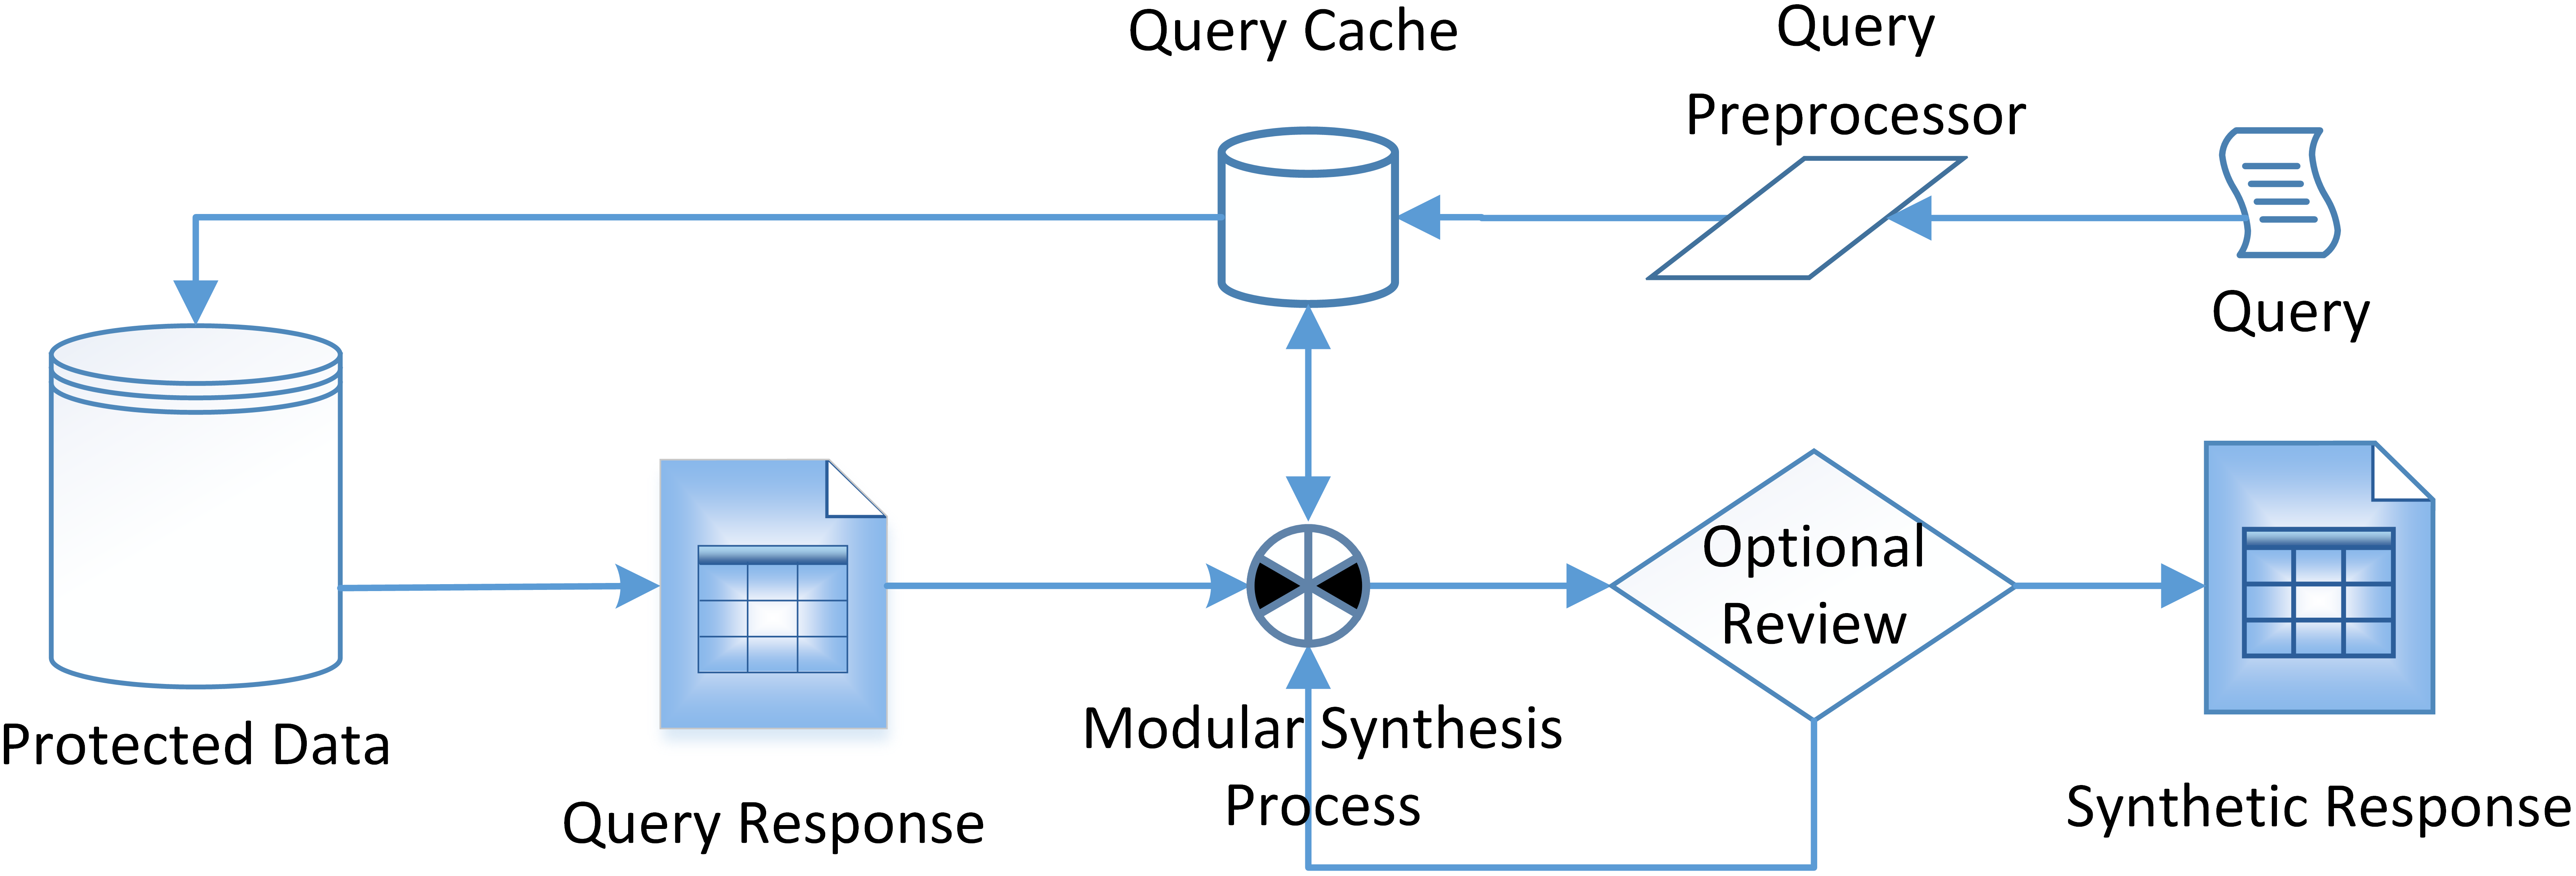
\includegraphics[width=\textwidth]{data_synthesis_process}


\section{Conclusion}

Basically need to put abstract here...


\bibliographystyle{unsrt}
\bibliography{bib}

\end{document}